\providecommand{\thebibpath}{..}
\makeatletter\def\input@path{{\thebibpath/}{.}}\makeatother
\documentclass[main.tex]{subfiles}
\begin{document}


	\todo[inline]{Write this properly}
	\begin{itemize}
		\item Try automatic differentiation
		\item Fully characterize the orientation of the sensor
		\item Try a quadratic controller
		\item Run more rollouts
		\item Try and encapsulate more of the matlab code
		\item $\cdots$
	\end{itemize}

	\section{The need for a quadratic controller}

	It seems than in doing the work needed to switch to the small unicycle, and the pause put in the project during that transition, much of the work by \citeauthor{queiro} was forgotten.
	In particular, they remark that a linear controller is insufficient in the sense of reaching a target position in \cite[fig.~8]{queiro}.
	We can go further, and prove that even symmetric upright balancing is not possible with a linear controller.
	Consider a stationary unicycle, with all states at the origin apart from pitch ($\psi$) and roll ($\theta$), and the action needed to stabilize it.
	Clearly, pitch can be stabilized by driving forward when leaning forward, and backwards when learning backwards.
	The decisions on how to control the turntable are more complex:
	\begin{description}
		\item[tilted forward and right ($\psi > 0, \theta > 0$)]
			Rotate clockwise ($\tau_t > 0$)\footnotemark.
		\item[tilted forward and left ($\psi > 0, \theta < 0$)]
			Rotate counter-clockwise ($\tau_t < 0$).
		\item[tilted backward and right ($\psi < 0, \theta > 0$)]
			Rotate counter-clockwise ($\tau_t < 0$).
		\item[tilted backward and left ($\psi < 0, \theta < 0$)]
			Rotate clockwise ($\tau_t > 0$).
	\end{description}
	\Cref{fig:balancing} shows both of these control schemes pictorially.
	The wheel controller in \cref{fig:balancing:wheel} can be described by $\tau_w = k\psi$, a linear controller.
	However, the turntable controller in \cref{fig:balancing:tt} requires a controller of the form $\tau_t = k\psi\theta$, a quadratic controller.
	While some success was shown using the linear controller in this and previous reports, this success can only ever hold when the robot stays within one half-plane of the pitch-roll state-space -- that is, always remains tilted forwards, or to one side.

	\begin{figure}
		\begin{subfigure}[t]{0.3\linewidth}
			\centering
			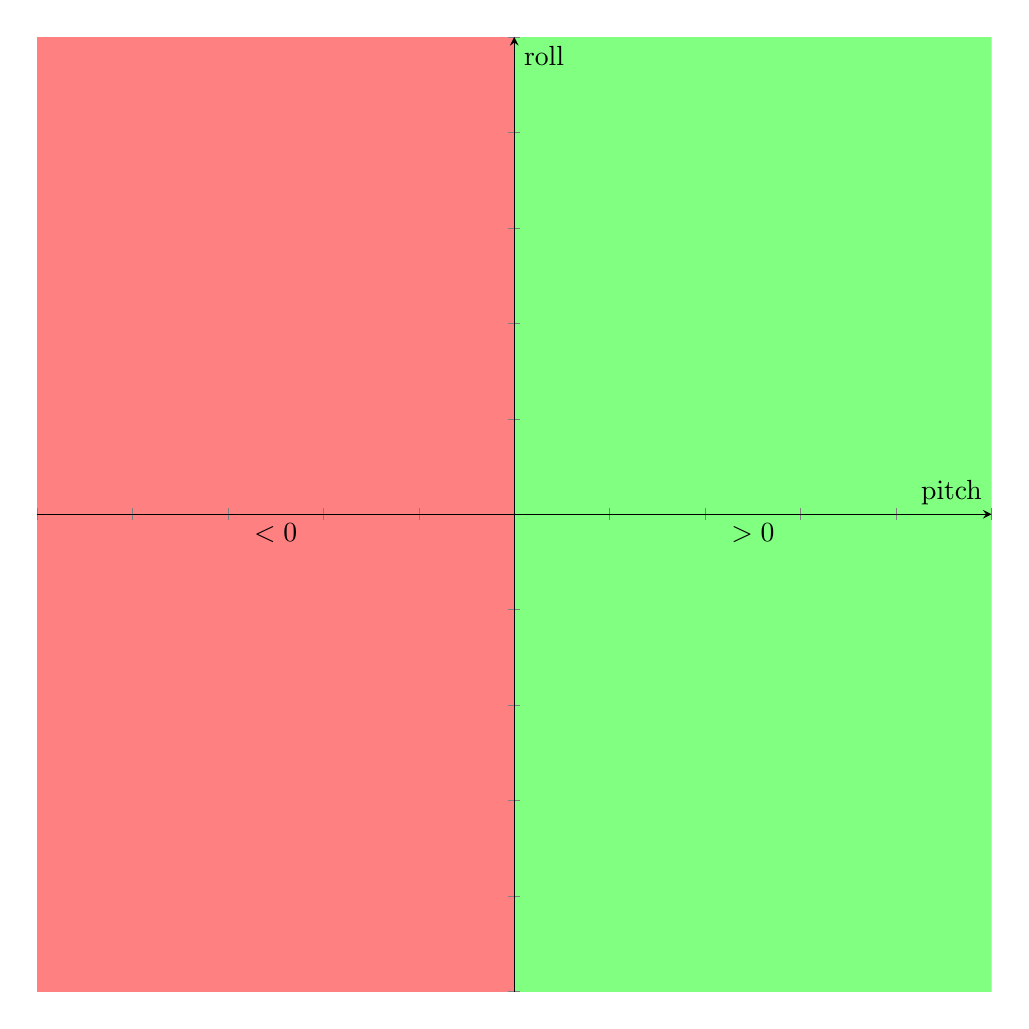
\begin{tikzpicture}
				\begin{axis}[%
					width=\linewidth,
					height=\linewidth,
					scale only axis,
					xmin=-1,xmax=1,
					ymin=-1,ymax=1,
					ylabel={roll},
					xlabel={pitch},
					xticklabels={{}},
					yticklabels={{}},
    				axis lines=middle,
    				axis on top=true
				]
					\fill[green!50]
						(current axis.above origin) rectangle (current axis.south east)
						node[black,midway, below] {$> 0$};
					\fill[red!50]
						(current axis.above origin) rectangle (current axis.south west)
						node[black,midway, below] {$< 0$};
				\end{axis}
			\end{tikzpicture}
			\caption{for $\tau_w$}
			\label{fig:balancing:wheel}
		\end{subfigure}\hfill
		\begin{subfigure}[t]{0.3\linewidth}
			\centering
			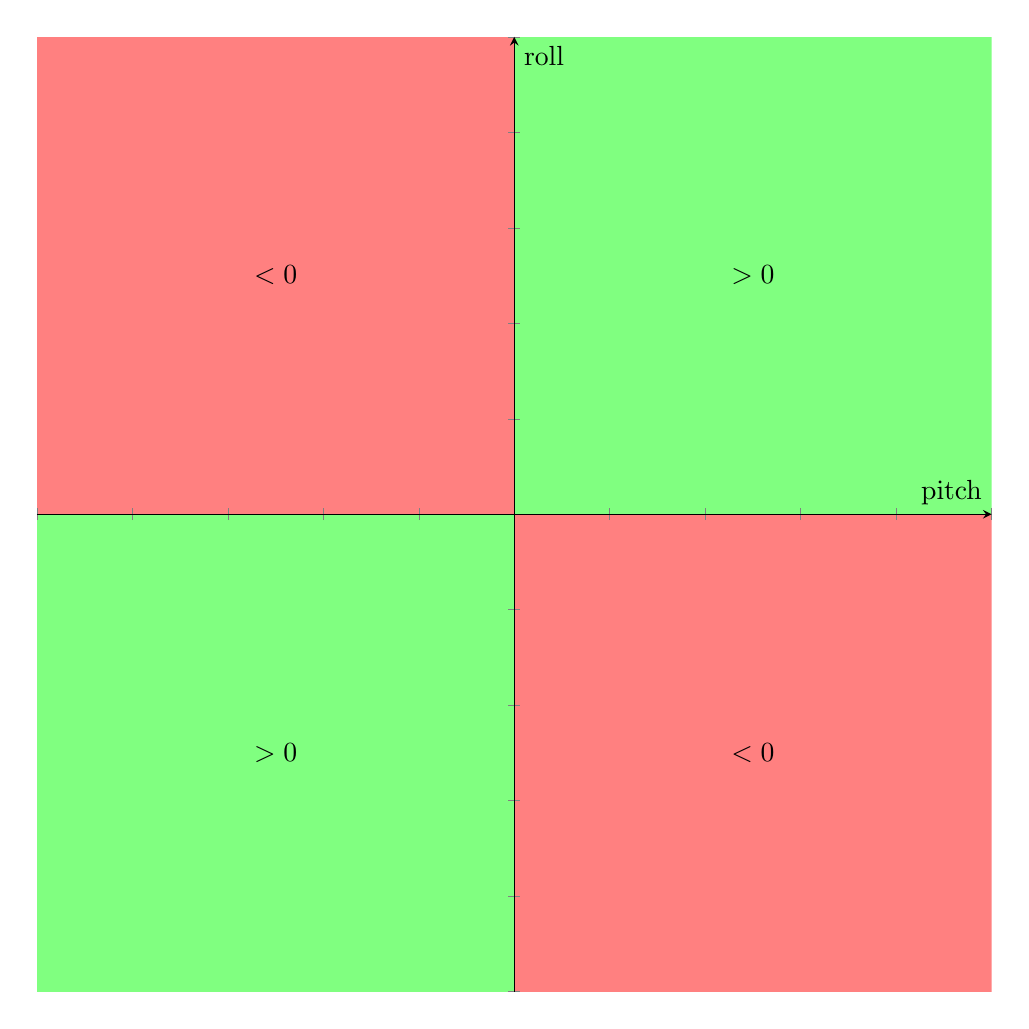
\begin{tikzpicture}
				\begin{axis}[%
					width=\linewidth,
					height=\linewidth,
					scale only axis,
					xmin=-1,xmax=1,
					ymin=-1,ymax=1,
					ylabel={roll},
					xlabel={pitch},
					xticklabels={{}},
					yticklabels={{}},
    				axis lines=middle,
    				axis on top=true
				]
					\fill[green!50]
						(current axis.origin) rectangle (current axis.north east)
						node[black,midway] {$> 0$};
					\fill[red!50]
						(current axis.origin) rectangle (current axis.north west)
						node[black,midway] {$< 0$};
					\fill[green!50]
						(current axis.origin) rectangle (current axis.south west)
						node[black,midway] {$> 0$};
					\fill[red!50]
						(current axis.origin) rectangle (current axis.south east)
						node[black,midway] {$< 0$};
				\end{axis}
			\end{tikzpicture}
			\caption{for $\tau_t$}
			\label{fig:balancing:tt}
		\end{subfigure}
		\caption{Controller required for stabilization}
		\label{fig:balancing}
	\end{figure}

	\footnotetext{Rotating the turntable counter-clockwise exerts a clockwise moment on the robot body}

\end{document}